\centerline{\bf \Large  6 класс}

\problem{\textbf{1}} Пюрвя Мучкаевич придумал систему перевода цифр в буквы и обратно, в которой каждой из десяти цифр соответствует одна уникальная буква. Он решил воспользоваться новой системой и умножил в столбик два слова УДЕ $\times$ УРАЛАН. Мог ли Пюрвя Мучкаевич получить в результате слово ЭРДНИЕВЫ? Если мог, то приведите пример таких чисел, если нет, то объясните почему.

\textbf{Решение:} Не мог получить, т.к. количество различных букв равно 11, а всевозможных цифр всего 10.

\textbf{Критерии.} \\
\textit{7 баллов} $-$ Полностью верное решение\\
\textit{0 баллов} $-$ Любое решение, в котором мог\\
\textit{0 баллов} $-$ Любой ответ без объяснений\\

\problem{\textbf{2}} Решите задачу:

а) В стране УДЕ есть песчаный берег длиной 50 метров, проходящий вдоль реки. Корабль длиной 10 метров проходит мимо берега за 3 секунды, если плывёт по течению, и за 5 секунд - если против. За сколько секунд бумажный кораблик доплывёт от одного конца берега до другого?

б) Составьте и решите обратную задачу по схеме: 50; ?; 3; 5; 12,5.

\textbf{Решение А:} Чтобы проплыть мимо берега кораблю нужно будет еще и проплыть собственную длину. Поэтому корабль проплывает расстояние равное 60м. Тогда скорость по течению 60/3=20м/с, против течения 60/5=12м/с. Тогда разница этих значений и есть удвоенная скорость течения. (20-12)/2=4м/с. Бумажному же кораблику нужно проплыть от одного конца до другого, то есть 50м. Т.к. скорость бумажного кораблика равна скорости течения, то за 50/4=12,5с бумажный кораблик доплывёт от одного конца берега до другого.

\textbf{Примерное условие Б:} В стране УДЕ есть песчаный берег длиной 50 метров, проходящий вдоль реки. Корабль неизвестной длины проходит мимо берега за 3 секунды, если плывёт по течению, и за 5 секунд - если против. Найдите длину корабля, если бумажный кораблик доплывёт от одного конца берега до другого за 12,5 секунд?

\textbf{Решение Б:} Скорость течения равна 50/12,5=4м/с. Пусть длина корабля равна $X$ метров, тогда составим уравнение: $\dfrac{50+X}{3}-\dfrac{50+X}{5}=2\cdot4$. Решая, которое получаем $X=10м$

\textbf{Критерии.} \\
\textit{0-4 баллов} $-$ Решение пункта А\\
\textit{0-1 балла} $-$ Составление условия пункта Б \\
\textit{0-2 баллов} $-$ Решение пункта Б\\
\textit{0 баллов} $-$ Любой ответ без объяснений\\

\problem{\textbf{3}} Фигура \textit{Сайгак} бьёт все клетки, находящиеся от неё через клетку слева, справа, сверху или снизу, а также бьёт клетку, на которой стоит. Какое наименьшее количество \textit{Сайгаков} необходимо поставить на клетчатую доску 8 × 8 , чтобы эти фигуры били все клетки доски?

\textbf{Решение:} Раскрасим клетки доски в 4 цвета следующим образом: все клетки, куда может прийти Сайгак из, не умаляя общности, левой нижней угловой клетки, покрасим в первый цвет. Сдвигами этого множества клеток вправо, вверх и вправо вверх получаем 4 множества клеток. Рассмотрим одно из них. Чтобы все клетки были побиты, нужно как минимум 4 Сайгака, так как каждый из них бьет не более 5   клеток, и, следовательно, 3 и меньше Сайгаков бьют максимум 15 клеток. Пример расстановки 4   Сайгаков: выделим 4   непересекающихся Т-образных фигур, в каждой из которых отметим по одному Сайгаку. И так как Сайгак, стоящий на клетке из одного множества, не может дойти до клеток из трех других, получаем, что всего нужно как минимум 16 Сайгаков.

\begin{center}
    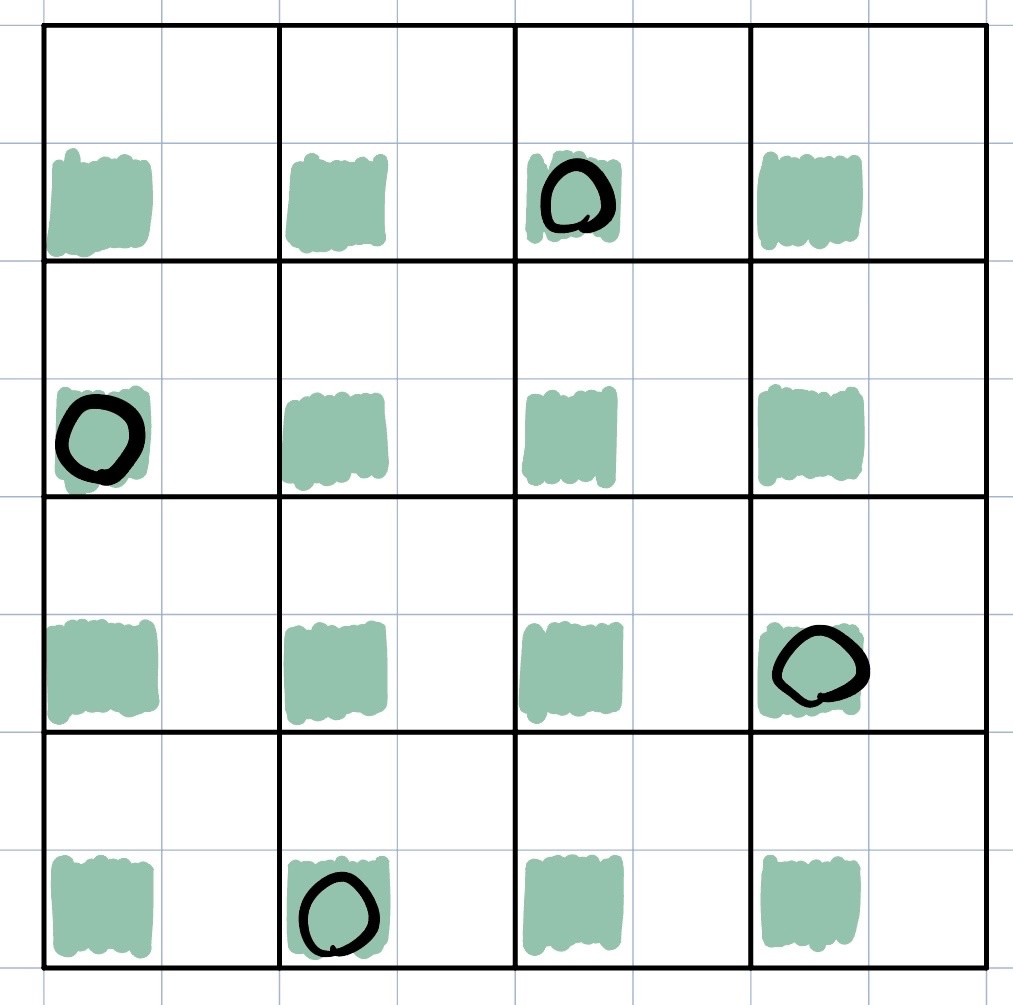
\includegraphics[width=0.3\textwidth]{Секретная информация/УДЕ 2024-2025/Регион. Решения/4.5_5.4_6.3.png}
\end{center}

\textbf{Критерии.} \\
\textit{2 балла} $-$ 16 сайгаков без объяснений\\
\textit{1 балл} $-$ Меньше 16 сайгаков без объяснений\\
\textit{0 баллов} $-$ Больше 16 сайгаков без объяснений\\
\textit{0-5 баллов} $-$ Поиск примера и оценка\\

\problem{\textbf{4}} Во дворе у Батыра есть три закрытых загона с номерами 1, 2 и 3. В одном из них 1 коричневый, 1 чёрный и 1 белый ягнёнок, в другом - 1 коричневый и 1 белый, в третьем - 1 чёрный ягнёнок. При этом известно, что номер загона не совпадает с числом ягнят внутри загона. Как, узнав цвет только одного ягнёнка из одного загона, найти число ягнят в каждом загоне?

\textbf{Решение:} Узнаем цвет ягнёнка из 3 загона. В 3 загоне может быть 2 ягнёнка или 1, при этом сколько на самом деле ягнят определяется однозначно благодаря различным цветам (поэтому не узнаем цвет из других загонов). Если в 3 загоне 2 ягнёнка, то в 1 уже не может быть 2, а это значит, что в 1 загоне - 3 ягнёнка и во 2 загоне - 1 ягнёнок. Если же в 3 загоне 1 ягнёнок, то во 2 уже не может быть 1, а это значит, что во 2 загоне - 3 ягнёнка и в 1 загоне - 2 ягнёнка. 

\textbf{Критерии.} \\
\textit{1 балл} $-$ В первом 2 или 3, во втором 1 или 3 и в третьем 1 или 2 ягнёнка\\
\textit{0-2 балла} $-$ Однозначное определение последующих загонов, если знаешь любой один\\
\textit{0-4 балла} $-$ Подходить нужно к третьему (однозначное определение по цветам)\\
\textit{0-7 баллов} $-$ Полный перебор\\
\textit{0 баллов} $-$ Любой ответ без объяснений\\

\problem{\textbf{5}} В стране УДЕ мальчики днём всегда говорят правду, а ночью всегда лгут, а девочки — наоборот. Днём каждый из них сказал: “У меня знакомых мальчиков на 1 больше, чем знакомых девочек”, а ночью — “Среди незнакомых мне жителей страны мальчиков на 1 больше, чем девочек”. Могло ли в стране УДЕ быть ровно 2025 жителей?

\textbf{Решение:} Для решения задачи полезно знать следующий факт, который мы для удобства сформулируем в терминах знакомства. Не существует компании, состоящей из нечётного числа людей, в которой каждый человек имеет нечётное количество знакомых (среди людей из этой компании).

Доказательство. Пусть все знакомые пожмут друг другу руки. Так как в каждом рукопожатии участвуют две руки, значит, суммарное количество «протянутых рук» чётно. С другой стороны, каждый человек протягивал руку нечётное число раз, чтобы суммарное число «протянутых рук» в этой ситуации получилось чётным, число людей должно быть чётным.

Каждый мальчик днём говорил правду, значит, у него нечётное число знакомых (поскольку среди них мальчиков на 1 больше, чем девочек). А каждая девочка сказала правду ночью, и по той же причине у неё нечётное число незнакомых.

Предположим, что в стране 2025 жителей. Тогда у каждого человека сумма количества знакомых и незнакомых равна 2024 (чётное число). Следовательно, у каждого человека количество знакомых имеет ту же чётность, что и количество незнакомых.

Таким образом, у каждой девочки нечётное количество незнакомых и, следовательно, нечётное количество знакомых. В итоге получаем, что каждый из 2025 жителей, имеет нечётное число знакомых, чего быть не может.

\textbf{Критерии.} \\
\textit{0-5 баллов} $-$ Продвижение через идеи чётности\\
\textit{1 балл} $-$ Лемма о рукопожатиях без доказательства\\
\textit{1 балл} $-$ Доказательство леммы о рукопожатиях\\
\textit{0 баллов} $-$ Любой ответ без объяснений\\